\chapter{Análise Exploratória Dados}
\label{chp:AnaliseDados}

\section{\textit{Dataset} em estudo}
\label{sec:DatasetEstudo}

Como referido, neste projeto procura-se utilizar as capacidades de generalização de uma \textit{Rede Neuronal Artificial} para a identificação do nível emocional de uma determinada publicação, com base nas palavras utilizadas na sua composição.  

Como suporte de dados para o processo de treino e teste da rede, foi utilizado um \textit{dataset} com informações de publicações da rede social \textit{Twitter}, recolhidas num período entre 1 de janeiro de 2016 e 31 de Julho de 2017. 
Será sobre este conjunto de dados que recai a fase de pré processamento de dados, abordada ao longo deste capítulo.

Como principais atributos, o referido \textit{dataset} apresenta inicialmente os campos:

\begin{itemize}
    \item \textbf{\textit{UserLocation}} – (\textit{String}) Representação textual da localização do utilizador que realizou a publicação. 
    A localização toma a forma de uma string, geralmente com o nome da cidade e o país. Pode também apresentar apenas as coordenadas de longitude e latitude ou valores nulos;
    
    \item \textbf{\textit{IdPost}} – (\textit{Inteiro}) Identificador único de cada uma das publicações;
    
    \item \textbf{\textit{TextPost}} – (\textit{String}) Conteúdo textual da publicação. 
    Apresenta a informação relevante que se procura analisar, após pré tratamento e adaptação, com base em RNAs;
    
    \item \textbf{\textit{Hashtags}} – (\textit{String}) Conjunto de \textit{hashtags} utilizadas junto da publicação. 
    
    Num sentido de uniformização, no contexto do \textit{dataset} identifica-se por "\textit{hashtags}" o conjunto de palavras iniciadas pelo carácter $\#$ e que procuram identificar as palavras chave ou tópicos da publicação. 
    
    Este campo pode encontrar-se vazio (valores nulos) ou conter um conjunto de um ou mais \textit{hashtags};
    
    \item \textbf{\textit{Date}} – (\textit{Data}) Registo da data em que a publicação foi colocada online, segundo o formato "Dia/Mês/Ano Hora:Minutos". 
    
    Cerca de 279 instâncias contêm este atributo como nulo;
    
    \item \textbf{\textit{TweetLat}} – (\textit{Inteiro}) Valor da latitude na qual a publicação foi colocada online;
    \item \textbf{\textit{TweetLon}} – (\textit{Inteiro}) Valor da longitude na qual a publicação foi colocada online;
    
    \item \textbf{\textit{PhotoLat}} e \textbf{\textit{PhotoLon}} – (\textit{Inteiros}) Valores da latitude e longitude associados à fotografia colocada junto com a publicação.
\end{itemize}

No total, o \textit{\textit{dataset}} é composto por um conjunto de 990473 instâncias. Nas seguintes secções serão destacadas as alterações realizadas ao dataset a nível de limpeza e criação de novos atributos. 

\section{Análise dos atributos}
\label{sec:AnaliseAtributos}

No sentido de identificar o nível emocional de uma publicação, foi inicialmente realizado um estudo aos dados fornecidos, no sentido de interpretar os seus valores e determinar qual a relevância de cada um dos atributos neste contexto.

Nesta secção, procura-se assim justificar a escolha dos atributos do dataset a as alterações que se realizaram ao mesmo. 
Tal como já referido, o conjunto de dados recolhidos resulta da recolha de um conjunto de informações associadas a diversas publicações na rede social \textit{Twitter}. 

\begin{multicols}{2}
\begin{itemize}
    \item \textit{UserLocation}
    \item \textit{IdPost}
    \item \textit{TextPost}
    \item \textit{Hashtags}
    \item \textit{Date}
    \item \textit{TweetLat / TweetLon}
    \item \textit{PhotoLat / PhotoLon}
\end{itemize}
\end{multicols}

O primeiro processo de filtragem de qualidade destes parâmetros baseia-se na presença de valores nulos, ou seja, no número de registo em falta para um determinado atributo. 
Nesse sentido, os atributos \textit{TweetLat, TweetLon, PhotoLat} e \textit{PhotoLon} foram automaticamente removidos, por apresentarem uma taxa de valores nulos de 100\%. 
Sendo valores inteiros, esta informação foi conseguida através de uma análise segundo a ferramenta \textit{Weka} (Figura \ref{fig:analiseWeka}).  

\begin{figure}[t]
    \centering
    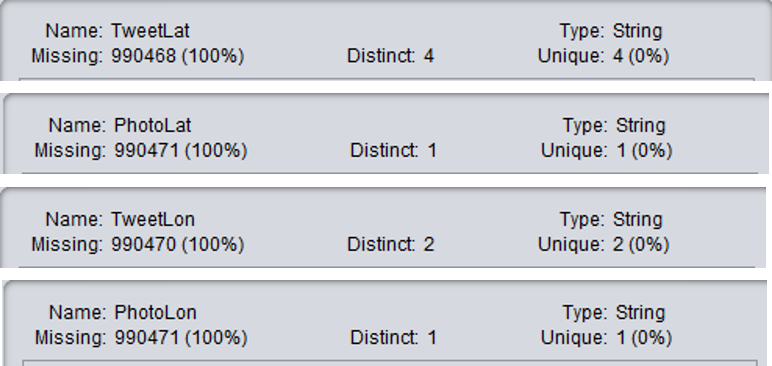
\includegraphics[scale=1]{Imagens/weka1.png}
    \caption{Análise do número de valores nulos e distintos dos atributos do dataset, recorrendo à ferramenta \textit{Weka}}
    \label{fig:analiseWeka}
\end{figure}

Sendo que por si só, a análise de linguagem natural já é um processo bastante dependente do contexto da frase e da forma como se organizam as palavras, uma das dificuldades associadas a este tipo de processamento recai na ambiguidade das palavras. 

Neste sentido, o uso de palavras soltas pode estar associado a diversos contextos emocionais ou até com formas de estilo como ironia. Por este motivo, foi tomada a decisão de ignorar quais \textit{hashtag} existente no dataset, dado que no contexto não apresentam um conhecimento sólido para o processo de aprendizagem da rede.

Assim, foi removida integralmente a coluna relativa ao atributo \textit{Hashtags}, que continha a listagem de eventuais \textit{hashtags} associados à publicação. 

O atributo \textit{IdPost} foi também removido nesta fase inicial de limpeza, dado que por ser único para cada publicação, não apresenta qualquer informação capaz de ser apreendida e generalizada pelo processo de aprendizagem da rede neuronal artificial. 

Os parâmetros \textit{UserLocation} e \textit{Date} foram mantidos por apresentarem alguma integridade nos seus valores. 
Numa fase posterior ao treino e teste de desempenho da RNA, estes registos podem eventualmente ser utilizados para gerar dados e estatísticas com base na localização do utilizador e o nível emocional da publicação. Contudo, não serão utilizados nem adaptados para o processo de treino da rede. 

Em suma, de todos os atributos do conjunto de dados, aquele que será exclusivamente adaptado para ser utilizado no processo de evolução da rede será o conteúdo textual da publicação, \textit{TextPost}, dado que é sobre este texto que se procura classificar o nível emocional da frase.

\section{Adaptação do \textit{Dataset}}
\label{sec:AdaptacaoDataset}

Como referido na secção anterior, a análise da semântica de um determinado texto está intrinsecamente ligado com o contexto em que a frase é composta e de que forma as palavras estão organizadas na mesma. 

Para um processo de análise de texto com base em algoritmos de \textit{Machine Learning}, registos com palavras soltas como os \textit{hashtags} ou hiperligações para páginas online, são alguns dos exemplos de informações que não apresentam nenhum material útil para o processo de extração de conhecimento. 

Relativamente a estes dois tipos de "palavras":
\begin{itemize}
    \item Analisar um \textit{hashtag} pelo valor da palavra em si, seria assumir de forma implícita um contexto para essa palavra e utilizar o peso da palavra nesse contexto em qualquer publicação onde esse \textit{hashtah} fosse utilizado.
    
    A titulo de exemplo, uma publicação com um contexto negativo e associado a tristeza pode apresentar um hashtag com a palavra \textit{"happy"}, meramente aplicada num contexto de ironia e como tal, oposta ao verdadeiro sentido emocional da publicação.
    
    Neste sentido, atribuir valor às palavras individuais dos \textit{hashtags} seria afetar o desempenho de classificação e enviesar a capacidade de análise de qualquer processo de aprendizagem que fosse utilizado. 
    
    Por este motivo, foram também removidos todos os \textit{hashtags} que surgissem no conteúdo textual da publicação. 
    Para isso foi simplesmente utilizada a ferramenta \textit{NotePad++} e utilizada a expressão regular \textit{\#( [a-zA-Z0-9] | [À-ÿ] )*} para apanhar todos os \textit{hashtags}. 
    
    \item Apesar de ser possível, a partir do endereço de uma hiperligação, utilizar uma API para extrair todas as palavras-chave associadas ao conteúdo dessa página, a obtenção desta lista de palavras-chave levaria ao mesmo problema que os \textit{hashtags}, descrito no tópico anterior. 
    
    Como consequência, todas as referências a hiperligações foram também removidas do conteúdo do texto da publicação. 
    
    Contudo, a representação de \textit{urls} estava bastante fragmentada e incoerente, tendo mostrado alguma dificuldade numa completa limpeza dos mesmos. A solução passou pelo uso de expressões regulares mais complexas, criadas para o contexto e,  uso dos métodos do \textit{package Tweet PreProcessor} existentes em \textit{Python}. 
    
\end{itemize}

Focando no conteúdo da publicação que é efetivamente útil para análise, é relevante frisar que no \textit{dataset} fornecido não existe qualquer relação entre as frases das publicações e o valor emocional associado às mesmas. 

Dado que este projeto recai sobre o uso de RNAs segundo um paradigma de aprendizagem supervisionado, é necessário fornecer à rede um conjunto de dados de treino junto com o respetivo conjunto de \textit{labels}, que identifique qual o resultado de \textit{output} esperado para um cada \textit{input} de treino.

Para gerar estas informações é necessário recorrer àquilo que pode ser visto como um dicionário, que mapeia o valor de uma palavra com o nível de sentimento a si associado. 
Analogamente, a forma mais simples de medir o peso emocional de uma frase, recai também no uso destas estruturas, somando o peso das palavras que compõe uma frase.  

Para gerar esta métrica para cada uma das instâncias do dataset, foram tidas em conta as seguintes considerações: 

\begin{itemize}
    \item O dataset é composto por publicações em diversas linguagens, nomeadamente inglês, francês e italiano;
    
    \item Utilizar as instâncias apenas com publicações em inglês seria reduzir significativamente o volume do \textit{dataset} e, com isso, perder informação relevante para o processo de aprendizagem da rede; 
    
    \item Não sendo viável remover todas as publicações que não se encontrem em inglês e dado que a maioria dos dicionários <Palavra, Valor-Emocional> existentes e disponíveis recaem na terminologia inglesa, uma das soluções passa pela tradução de todos as instâncias para a inglês. 
    
    Contudo, recorrendo à API de tradução disponibilizada pela plataforma \textit{Google Translate} \cite{googleTransAPI}, o processo de tradução é implementado sobre pedidos http. 
    Cada pedido envolve o encapsulamento (\textit{marshling e unmarsheling}) de pacotes \textit{JSON} com o conteúdo e resposta da tradução, pelo que o tempo de cada tradução andava acima de 1 segundo por frase/publicação. 
    
    Dado o tempo disponível para este projeto e a dimensão do dataset (+ de 900 mil instâncias), a opção de traduzir cada publicação não se apresenta viável;
\end{itemize}

A solução encontrada passou pelo uso de uma nova API de mapeamento <Palavra, Valor-Emocional> que fosse capaz de lidar com várias linguagens, evitando assim que fosse necessária uma tradução prévia do conjunto de dados. 

É com base neste nível de sentimento, quantificado num valor numérico, que se mapeia o peso emocional das frases de uma publicação numa das seguintes classes:

\begin{multicols}{3}
\begin{itemize}
    \item \textit{Negativo}
    \item \textit{Neutro}
    \item \textit{Positivo}
\end{itemize}
\end{multicols}

Apesar do enunciado do projeto especificar que as classes de classificação da RNA deveriam ser apenas $"\textit{Negativo}"$ ou $"\textit{Positivo}"$, foi tomada a decisão que a classificação seria mais coerente e rigorosa de existisse também o nível \textit{Neutro}.

Desta forma, a \textit{tag} $"Neutro"$ procura representar as publicações que não apresentam qualquer nível sentimental, seja porque o seu conteúdo é ambíguo de interpretar ou porque são frases simples, que procuram apenas descrever factos ou eventos. 

Pelo facto de uma frase não ser simplesmente positiva ou negativa, justifica-se assim a decisão de existirem 3 classes de previsão. 


\section{Criação de Atributos \textit{Target/Output}}
\label{sec:CriacaoTarget}

Para a criação deste novo atributo, que representa o output sobre o qual a rede deve treinar e ser capaz de realizar previsão, foram exploradas algumas soluções de análise de texto já implementadas na linguagem \textit{Python}. 

Relativamente à escolha de uma API capaz de realizar uma análise em linguagem natural e deteção de sentimentos, foram exploradas as seguintes soluções:

\begin{itemize}
    \item \textbf{\textit{Natural Language Toolkit - NLTK}} \cite{NLTK}: A plataforma \textit{NLTK} apresenta-se como uma das ferramentas \textit{Open-source} mais utilizadas para desenvolver algoritmos ou métodos que necessitem de analisar linguagem humana num contexto semântico. 
    
    No contexto de análise de sentimentos em frases, os métodos desta ferramenta baseiam-se em técnicas de Classificação hierárquica para determinar o nível de polaridade e subjetividade de uma frase. Por polaridade entende-se o nível de sentimento de uma frase (positivo ou negativo) e por subjetividade entende-se o nível de confiança da classificação, conforme o contexto e conteúdo da frase analisada. 
    
    A \textit{API} desenvolvida para \textit{Python} \cite{NLTK-python} apresenta como pontos positivos e facto de devolver a Polaridade dividida em dois valores decimais, para identificar a percentagem de sentimento negativo ou positivo na frase. 
    
    Contudo, o seu foco encontra-se ainda muito voltado para a língua inglesa, tornando-a assim inadequada para o dataset em análise, pelos motivos supracitados na listagem anterior. 
    
    \item \textit{\textbf{Microsoft Azure: Text Analytics AP}} \cite{azure}: Disponibilizados na plataforma \textit{Azure}, a Microsoft disponibiliza um conjunto de soluções que designa como "Serviços cognitivos" pela sua envolvência com a temática da inteligência artificial. 
    
    Estes serviços oferecem APIs para processamento de imagem, voz, conhecimento e linguagem. É nesta ultima área que surge a ferramenta \textit{Text Analytics} \cite{azureAPI}.
    
    Esta solução é capaz de, para uma determinada entrada de texto, automaticamente determinar a sua linguagem e devolver o seu nível de sentimento, junto com uma lista de palavras chave/\textit{target} que permitem atribuir um determinado nível de sentimento à frase. 
    
    Apesar da ferramenta funcionar com um grande número de linguagens e apresentar uma elevada capacidade de análise para frases com palavras relacionadas entre si, a chave de utilização deste serviço é limitada a 30 dias e a 5000 pedidos por dia. 
    
    Novamente, a exploração integral do dataset com esta API seria impossível, devido ao seu volume de dados e ao domínio temporal deste projeto. 
    
    \item \textit{\textbf{TextBlob}} \cite{textblob}: Procurando contornar as limitações encontradas nas duas ferramentas anteriores, a biblioteca \textit{TextBlob} apresenta-se como a solução encontrada para pré processar o dataset limpo, como forma de calcular o nível de sentimento de cada frase. 
    
    Esta plataforma é construida sobre a ferramenta \textit{NLTK} referida no primeiro ponto, embora acrescente sobre os seus métodos a capacidade de deteção de sentimentos em texto em várias linguagens nativas. 
    
    Por este motivo e, sendo totalmente \textit{open-source} e sem limite de pedidos, esta solução foi a utilizada para calcular os valores de sentimento de cada frase, sobre os quais a rede deve treinar e aprender a classificar/prever futuras frases de publicações. 

\end{itemize}

O uso da ferramenta \textit{TextBlob} envolve assim a tradução de publicações num idioma estrangeiro para inglês nativo, realizando uma tradução estocástica \cite{RepresentacaoTexto}. 

Considerando assim os resultados devolvidos pelos métodos da API \textit{TextBlob} para \textit{Python}, foram então acrescentadas duas colunas ao dataset:
\begin{itemize}
    \item A coluna \textbf{Polaridade}, que indica o nível de sentimento de um texto. 
        
    Toma valores decimais entre [-1, 1], sendo que frases com valores de polaridade próximos de -1 apresentam um conteúdo negativo e frases com valores de polaridade próximos de 1, associam-se a sentimentos positivos. 
        
    \item A coluna \textbf{Subjetividade}, onde se quantifica a confiança do nível calculado para o texto, conforme o seu contexto. 
        
    Toma valores decimais entre [0,1], sendo que valores próximos de 0 estão associados a textos bastante objetivos -nível de sentimento concreto para o contexto- e valores próximos de 1, recaem sobre textos subjetivos,onde a medição do nível de sentimento não é concreta para o contexto.
\end{itemize}

Relembrando que se procura classificar o nível emocional de uma frase apenas em três classes concretas (Secção \ref{sec:AdaptacaoDataset}), é necessário realizar uma descriterização dos valores tomados pelo atributo Polaridade. 
Uma vez que a API fornece duas métricas relevantes, foi tomada a decisão de conjugar estas duas informações num único atributo, que mapeia os valores dentes os parâmetros Polaridade e Subjetividade para uma das classes objetivo: Negativo, Neutro ou Positivo.  

Como forma de não criar tendências no processo de aprendizagem, nem classificar como positiva ou negativa frases com conteúdo/contexto ambíguo, foi tomada a decisão que todas as instâncias com subjetividade superior a 0.5 representam publicações com um conteúdo neutro. 

Para os restantes casos, onde exista pelo menos 50\% de certezas face à objetividade da publicação e ao seu contexto, o mapeamento do valor da polaridade para uma das três classes referidas foi realizado dividindo o intervalo de valores deste atributo de forma linear. 
A figura \ref{fig:niveisSentimento} procura descrever esquematicamente esta divisão. 

\begin{figure}[t]
    \centering
    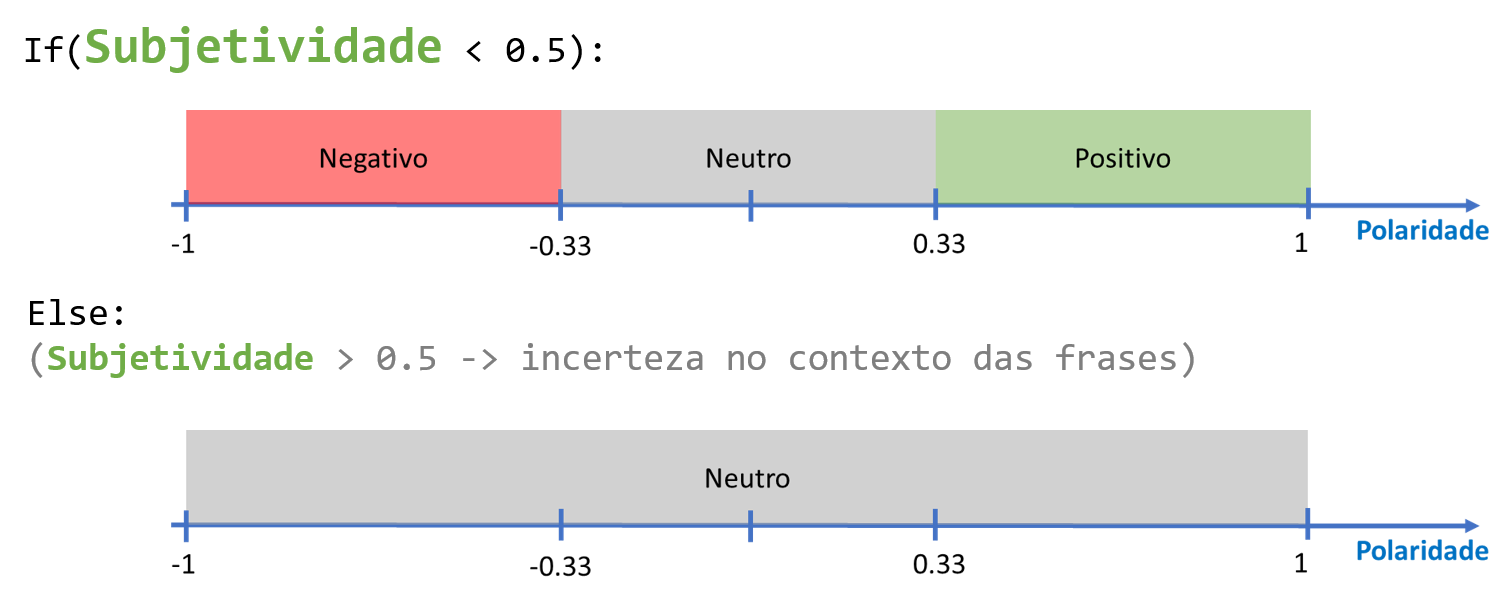
\includegraphics[scale=0.5]{Imagens/niveisSentimento.png}
    \caption{Mapeamento dos valores de polaridade e subjetividade para as classes "Negativo", "Neutro" e "Positivo". }
    \label{fig:niveisSentimento}
\end{figure}

Conjugando os resultados da API \textit{TextBlob} com o mapeamento acima referido, foi possível observar que uma massiva maioria dos casos foi identificada apenas com um valor neutro de sentimentos. (Figura \ref{fig:medidas})
Apenas cerca de 8\% das instâncias do dataset foram identificadas como associadas a um sentimento negativo/positivo. 

Sendo que as outras APIs de classificação textual, possíveis de utilizar para criar o atributo \textit{target}, se baseiam nos mesmo processos de classificação de linguagem natural, conclui-se que o dataset pode não ser o melhor para treinar de forma viável uma RNA, devido à discrepância entre casos neutros com os casos associados a sentimentos negativos/positivos. 

\begin{figure}
    \centering
    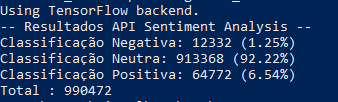
\includegraphics{Imagens/medidas.png}
    \caption{Percentagens de publicações classificadas num determinado nível de sentimento: Negativo, Neutro ou Positivo. }
    \label{fig:medidas}
\end{figure}

\section{Redução Dataset}
\label{sec:reducaodataset}

Tendo sido observado que o volume inicial do dataset se apresentaria como uma entrave para a construção de RNAs mais complexas e de maiores dimensões, foi tomada a decisão de reduzir significativamente o número de casos utilizados no processo de aprendizagem da rede. 

Uma vez que a manipulação do conjunto de dados completo implicaria recursos de memória e tempo de processamento não disponíveis no decorrer deste projeto, foram assim criadas a partir dele cerca de 100 mil instâncias para Treino e Teste das RNAs. 
Este novo dataset, apesar de conter cerca de $\frac{1}{10}$ do volume inicial, apresenta ainda assim uma quantidade significativa de casos, filtradas com mais detalhe e rigor a nível de tradução para a língua inglesa. 

Neste conjunto de dados foram selecionados 100 mil casos aleatórios do dataset inicial. 
Como pré processamento adicional, foi dado ênfase à limpeza de palavras com caracteres desconhecidos e referências a conteúdos sem informação útil para o processo de aprendizagem. 
Além disso, foi ainda utilizada a API do \textit{Google Translator} para realizar a tarefa de tradução cuidada dos \textit{tweets}. (No dataset completo não foi possível usar esta ferramenta devido ao tempo de tradução do dataset inteiro)

Esta redução permite aumentar a complexidade da rede, a nível de camadas intermédias e número de \textit{Epochs}, levando à possibilidade de mais cenários de treino/teste de RNAs. 
Ao utilizar-se um dataset de menores dimensões, o tempo de aprendizagem da rede e recursos necessários para representar os \textit{tweets} do dataset em formato de input da rede são significativamente menores.
